Интерфейс приложения организует работу с ассистентом. Для реализации доступного в использовании приложения был использован 
"гештальт-дизайн" \cite{wertheimer1938laws}, задающий правила композиции элементов интерфейса. Также были учтены
стандарты WAI-ARIA \cite{craig2009accessible}, задающие правила высокого контраста и выраженности контуров, позволяющих выполнять навигацию слабовидящим людям. 
Функционал приложения ограничено доступен и незрячими людям, использующим специальные приложения для аудио-отображения содержания сайта.

\begin{figure}[h]
    \centering
    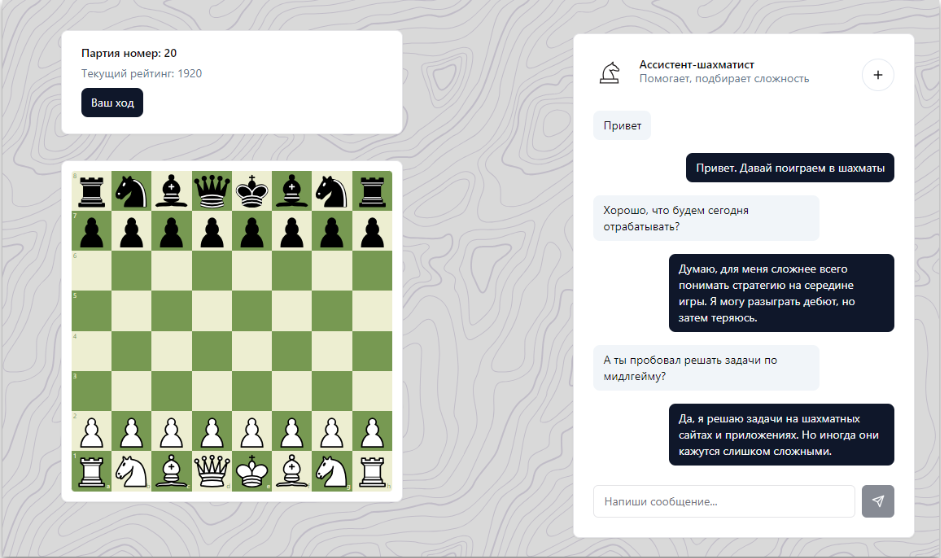
\includegraphics[width=0.7\textwidth]{assets/work/games/interface.png}
    \caption{Интерфейс имеет четкие и контрастные элементы взаимодействия. Доска для игры и диалоговое окно размещены совместно }
    \label{chess}
\end{figure}

Веб-приложение доступно при подключение через браузер по адресу доменного имени \url{www.mathema-online.xyz}. 
Безопасность соединения обеспечивается криптографической защитой и сертификатами, исключающими возможность подмены доменного имени.

Интерфейс реализован с помощью популярной библиотеки React для языка программирования JavaScript \cite{gackenheimer2015introduction}.
Такой подход позволяет дескриптивно описывать элементы вебсайта с событийной реакцией на взаимодействие с пользователем. 
Особенностью подхода является возможность использовать общедоступные профессионально подготовленные 
схемы интерфейсов в виде css-разметки.
